\newpage
\hypertarget{treeToModel vis}{}
\subsection{Vis Tree to Model Source}
\visHeader

\begin{itemize}

\item[$\blacktriangleright$] Create a \texttt{TransformationLanguage} package and open a new ECore diagram and built it as depicted in
Fig.~\ref{ea:transformerclass}. Remember, when defining attributes, operations, and parameters, you \emph{must} use either the drop-down menu or the
\texttt{`\ldots'} button when defining their types.\footnote{Review Part II for more key details of constructing a metamodel}

\begin{figure}[htpb]
\begin{center}
  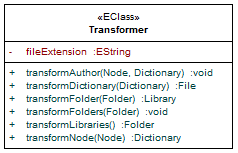
\includegraphics[width=0.5\textwidth]{ea_transformerClass}
  \caption{figureCaption}
  \label{ea:transformerclass}
\end{center}
\end{figure}

\item[$\blacktriangleright$] We can now specify a transformation TGG between \texttt{Dictionary} and \texttt{TransformationLanguage}! Right click on
\texttt{DictionaryCodeAdapter} and create a new TGG Diagram.

\begin{figure}[htpb]
\begin{center}
  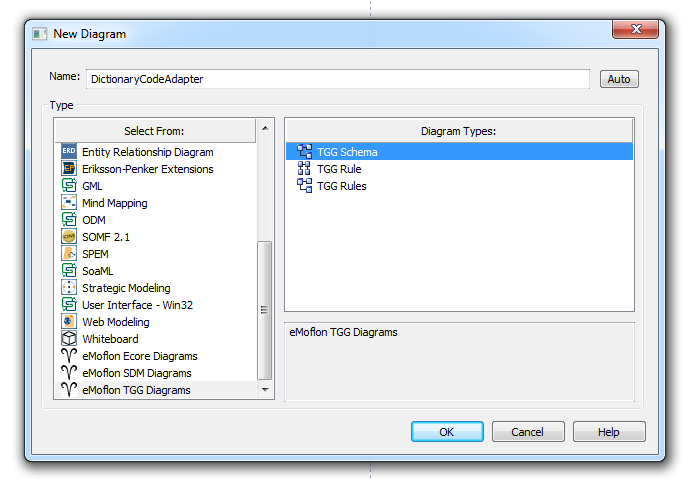
\includegraphics[width=0.5\textwidth]{ea_transformationTGGDiagram}
  \caption{figureCaption}
  \label{ea:transformerclass}
\end{center}
\end{figure}

\begin{figure}[htpb]
\begin{center}
  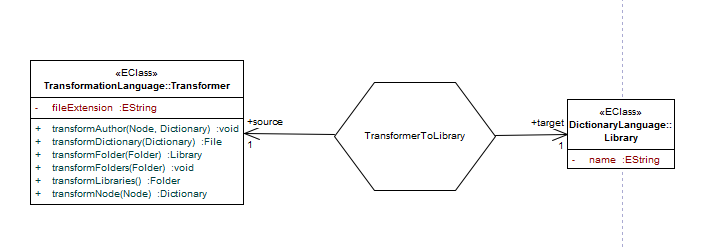
\includegraphics[width=0.5\textwidth]{ea_newTGGType}
  \caption{figureCaption}
  \label{ea:transformerclass}
\end{center}
\end{figure}

\begin{figure}[htpb]
\begin{center}
  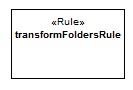
\includegraphics[width=0.5\textwidth]{ea_transformFoldersRuleDeclare}
  \caption{figureCaption}
  \label{ea:transformerclass}
\end{center}
\end{figure}


\end{itemize}
